\documentclass{article}

\usepackage{kbordermatrix}
\usepackage{amsmath}
\usepackage{tikz}
\usetikzlibrary{automata, positioning, arrows, calc}

\title{Frequentist and Bayesian Analyses of the Board Game \textit{Outlaw}}
\author{Jediah Katz}
\date{February 21, 2018}

\newcommand{\T}{\textbf{\textit{T}}}
\newcommand{\x}{\vec{x}}
\renewcommand{\arraystretch}{1.3}

\begin{document}
	\maketitle
	\pagenumbering{arabic}
	\begin{abstract}
		A variant of the dice-based board game \textit{Outlaw}, designed by Phil Horswell, was analyzed 
	\end{abstract}

	\section{Background}
	Two of the most prominent understandings of probability are the frequentist and Bayesian interpretations. Frequentist probability, most generally, defines probability as the relative frequency of an event's occurrence in a suitable number of repetitions of a process. In contrast, Bayesian probability, most generally, defines probability as the degree of confidence in an event's occurrence held by a suitable agent. Each of these interpretations of probability corresponds to its own means of modeling a process in order to determine the probability that particular events will occur.
	
	\subsection{Monte-Carlo Simulations}
	Imagine a rather boring game in which a single player rolls one die each turn and adds its value to the the score, which begins at zero. The player wins if the score is greater than twenty after five turns, and loses otherwise. Suppose we are interested in determining the probability that the player wins the game. In the frequentist interpretation of probability, an intuitive solution is to simply play the game many times, recording whether the player wins or loses.
	
	However, it is often impractical and time-consuming to manually repeat this process a suitable number of times in order for the relative frequency to converge. Fortunately, the use of a computer can greatly speed up the repetition of trials. By creating a simulation to model the playing of a game, millions of trials can be run in very little time, a process known as the Monte-Carlo method.
	
	It is worth noting that assumptions must often be made in the process of building a computer simulation. For example, in order to simulate the rolling of a die, we assume that a uniform pseudo-random number generator that generates integers in the interval {[1,6]} correctly models the behavior of a die.
	
	\subsection{Absorbing Markov Chains}
	For some more complex processes, however, even a computer simulation may not be feasible. Events with very low probability, such as ten dice each rolling a six, can easily require hundreds of millions of trials to occur in a simulation. Fortunately, Bayesian methods of probability modeling provide an elegant solution to this problem. As Bayesian probability is not constrained by the idea of frequency, we can use our assumptions to mathematically model processes.
	
	One of the most valuable tools for modeling in the Bayesian's belt is the Markov chain. A Markov chain is defined as a sequence of random variables $X_1, X_2, \ldots$ that describe the probabilities of transitions through a state space. Crucially, the process described by a Markov chain must fulfill the Markov property, also known as memorylessness; that is, the probability of transitioning from one state to another is independent of past states.

	A Markov chain on a finite state space $\Omega$ can be conveniently described by a transition matrix $\T$, an $|\Omega| \times |\Omega|$ square matrix such that $\T_{R, S}$ is the probability of transitioning from $R$ to $S$ for any two states $R, S \in \Omega$. Note that $\T$ is a right stochastic matrix, meaning that the probabilities in each row of $\T$ sum to 1. 
\\
	
	An absorbing Markov chain is simply a Markov chain for which there exists a state $S \in \Omega$ such that $\T_{S,S} = 1$. Equivalently, an absorbing Markov chain contains at least one state from which transition to another state is impossible. Absorbing Markov chains are especially useful for modeling games, as winning a game is typically an absorbing state.
	
	Consider the game represented by the directed graph below. The player begins at state $A$. Each turn, the player rolls a die and then transitions across the corresponding edge, if one exists. The player wins upon reaching state $C$.
	
	\[
	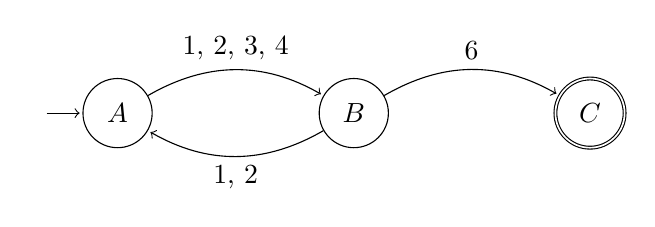
\begin{tikzpicture}[shorten >=1pt, node distance=3cm,auto, initial text={}]
      \node[state,initial] (a) {$A$};
      \node[state] (b) [right of=a] {$B$};
      \node[state,accepting] (c) [right of=b] {$C$};
      \path[->]
                (a) edge[bend left] node {1, 2, 3, 4} (b)
                (b) edge[bend left] node {6} (c)
                (b) edge[bend left] node {1, 2} (a);
     \end{tikzpicture}
	\]
	
	Since the probability of transitioning between states only depends on the current state, this game is an ideal candidate for a Markov chain. The state space $\Omega$ is $\{A, B, C\}$. We can represent the transition matrix $\textbf{T}$ as the following matrix:
	
	\[\kbordermatrix{~ &A & B & C \cr
		A&\frac{2}{6} &  \frac{4}{6}  & 0 \cr
		B& \frac{2}{6}  &  \frac{3}{6} & \frac{1}{6} \cr
		C& 0 & 0 & 1}\]
	
	At this point, it is very simple to determine the probability that the player is at any state in $\Omega$ after some number of turns. 

Let $\x$ be the initial state vector, a row vector such that $\x_A = 1$ for the initial state $A$ and $\x_B = 0$ for any other state $B \in \Omega$. Let $\Pr_S(n)$ refer to the probability of being at state $S$ after $n$ turns for some state $S \in \Omega$. We establish the following identity:
	$${\Pr}_S(n) = [\x (\T^{n})]_S$$
	
	
	By the associative property, this is equivalent to multiplying the initial state vector by the transition matrix $n$ times. Note that by multiplying the probability of being at each state $S \in \Omega$ by the probability of transitioning from $S$ to some other state $R \in \Omega$, and then summing these products, we obtain the probability of being at $R$ on the next turn. By multiplying $\x$ and $\textbf{T}$, we are repeating this process for each $R \in \Omega$.
	
	Returning to our game, we can use this identity to determine the probability of being at each state after ten turns. Note that the player begins at state $A$, so the initial state vector $\x$ is the one-hot row vector $
	[\begin{smallmatrix}
	1 & 0 & 0
	\end{smallmatrix}]
	$.
	
	\[{\Pr}(20) = 
	\begin{bmatrix}
	{\Pr}_{A}(20) & {\Pr}_{B}(20) & {\Pr}_{C}(20)
	\end{bmatrix} =
	\begin{bmatrix}
	1 & 0 & 0
	\end{bmatrix}
	\begin{bmatrix}
		\frac{2}{6} & \frac{4}{6} & 0           \\
		\frac{2}{6} & \frac{3}{6} & \frac{1}{6} \\
		0           & 0			  & 1
	\end{bmatrix}
	^{10}
	\]
	\[
	=	
	\begin{bmatrix}
	\frac{1033729}{7558272} & \frac{3486025}{15116544} & \frac{3187687}{5038848}
	\end{bmatrix}
	\approx \begin{bmatrix}
	.14 & .23 & .63
	\end{bmatrix}
	\]
	
	\begin{thebibliography}{9}
		\bibitem{interpretations}
		H\'{a}jek, Alan, ``Interpretations of Probability'', The Stanford Encyclopedia of Philosophy (Winter 2012 Edition), Edward N. Zalta (ed.), \texttt{https://plato.stanford.edu/archives/win2012/entries/probability-interpret/}.
	\end{thebibliography}
\end{document}